\documentclass[tikz,border=5pt]{standalone}
\usepackage{amsmath,amssymb}
\usetikzlibrary{trees}
\begin{document}
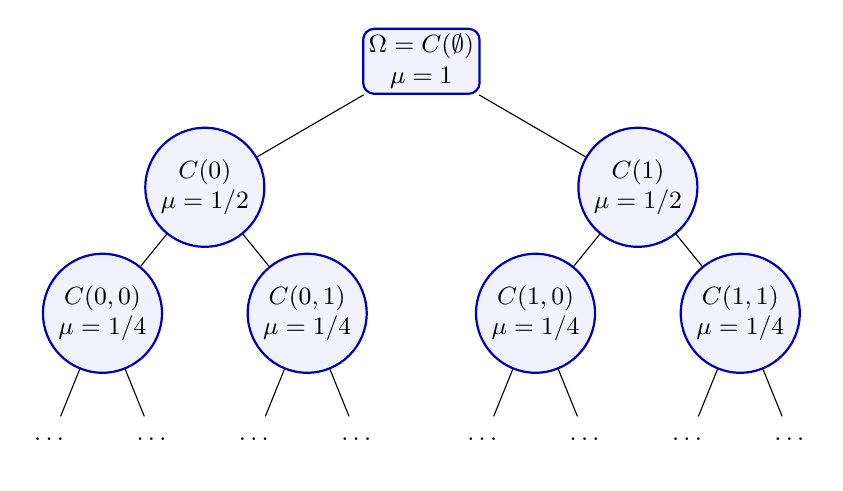
\begin{tikzpicture}[
    >=latex, font=\small,
    level 1/.style={sibling distance=5.5cm, level distance=1.6cm},
    level 2/.style={sibling distance=2.6cm, level distance=1.6cm},
    level 3/.style={sibling distance=1.3cm, level distance=1.6cm},
    every node/.style={circle, draw=blue!70!black, fill=blue!5, thick, inner sep=2pt, align=center}
  ]
  \node[rectangle, rounded corners] {$\Omega = C(\emptyset)$\\$\mu = 1$}
    child {
      node {$C(0)$\\$\mu = 1/2$}
      child {
        node {$C(0,0)$\\$\mu = 1/4$}
        child { node[draw=none, fill=none] {$\dots$} }
        child { node[draw=none, fill=none] {$\dots$} }
      }
      child {
        node {$C(0,1)$\\$\mu = 1/4$}
        child { node[draw=none, fill=none] {$\dots$} }
        child { node[draw=none, fill=none] {$\dots$} }
      }
    }
    child {
      node {$C(1)$\\$\mu = 1/2$}
      child {
        node {$C(1,0)$\\$\mu = 1/4$}
        child { node[draw=none, fill=none] {$\dots$} }
        child { node[draw=none, fill=none] {$\dots$} }
      }
      child {
        node {$C(1,1)$\\$\mu = 1/4$}
        child { node[draw=none, fill=none] {$\dots$} }
        child { node[draw=none, fill=none] {$\dots$} }
      }
    };
\end{tikzpicture}
\end{document}
